
%{{{ Preamble

\documentclass[journal,a4paper]{IEEEtran}

%{{{ Packages

\usepackage[l2tabu,orthodox, abort]{nag}
\usepackage{fontspec}

\usepackage{microtype}
\frenchspacing

\usepackage{polyglossia}
\setdefaultlanguage{english}

\usepackage{graphicx}
\graphicspath{{../material/paper/}{../material/background/}}

\usepackage{minted}
\usepackage{lipsum}
\usepackage{url}
\usepackage{stfloats}
\fnbelowfloat




\makeatletter
\let\MYcaption\@makecaption
\makeatother
\usepackage[font=footnotesize]{subcaption}
\makeatletter
\let\@makecaption\MYcaption
\makeatother

%}}}


%{{{ New commands

%\newcommand{\source}[1]{{\caption{\tiny {\fontspec{ProFontWindows} {Source: #1} } } } }
\newcommand{\source}[1]{Source: #1}
%}}}


%{{{ Avebritations

\def\krste/{Krste Asanovi\'c}
%\def\CC/{C\nolinebreak\hspace{-.05em}\raisebox{.4ex}{\tiny\textbf{+}}\nolinebreak\hspace{-.03em}\raisebox{.4ex}{\tiny\textbf{+} } }
%}}}

%{{{ Some hacks

\hyphenation{op-tical net-works semi-conduc-tor}
\addto\captionsenglish{\renewcommand\tablename{Listing}} %Use the table environment for code listings
%}}}

%}}}



%{{{ inputfile

\usepackage{tikz}
\usetikzlibrary{arrows, decorations.markings}
\usetikzlibrary{positioning,shapes,shadows,calc,positioning}
\usetikzlibrary{decorations.pathreplacing,angles,quotes}
\usetikzlibrary{decorations.pathmorphing}
%\usetikzlibrary{fit}


% This part taken from http://www.texample.net/tikz/examples/double-arrows/
% Double Arrows a la Chef
% Author: Dominik Haumann

% for double arrows a la chef
% adapt line thickness and line width, if needed
%\tikzstyle{vecArrow} = [thick, decoration={markings,mark=at position
%   1 with {\arrow[semithick]{open triangle 60}}},
%   double distance=1.4pt, shorten >= 5.5pt,
%   preaction = {decorate},
%   postaction = {draw,line width=1.4pt, white,shorten >= 4.5pt}]
%\tikzstyle{innerWhite} = [semithick, white,line width=1.4pt, shorten >= 4.5pt]


%\tikzstyle{mynode} = [rectangle,rounded corners,draw=black,top color=white, bottom color=white!50,very thick, inner sep=1em, minimum size=3em, text centered]
%\tikzstyle{invnode} = [inner sep=0,minimum size=0]
%
%\tikzstyle{abstract}=[rectangle, draw=black, rounded corners, fill=blue!40, drop shadow, text centered, anchor=north, text=white, text width=3cm]
%\tikzstyle{comment}=[rectangle, draw=black, rounded corners, fill=green, drop shadow, text centered, anchor=north, text=white, text width=3cm]
%\tikzstyle{myarrow}=[->, >=open triangle 90, thick]
%\tikzstyle{line}=[-, thick]


\tikzset{font={\fontsize{8pt}{7}\selectfont}}
\tikzset{every picture/.append style={scale=0.1}}


\usepackage{etex} %% Cool Stuff, see http://tex.stackexchange.com/a/36721/69074 : \foreach \i in {0,...,\number\numexpr\memBlocks-1\relax}
\newcommand{\CC}{C\nolinebreak\hspace{-.05em}\raisebox{.4ex}{\tiny\bf +}\nolinebreak\hspace{-.03em}\raisebox{.4ex}{\tiny\bf +}}




%{{{ Extract Coordinates

% http://tex.stackexchange.com/a/179946/69074
\makeatletter
\def\extractcoord#1#2#3{%
  \path let \p1=(#3) in \pgfextra{%
    \pgfmathsetmacro#1{\x{1}/\pgf@xx}%
    \pgfmathsetmacro#2{\y{1}/\pgf@yy}%
    \xdef#1{#1} \xdef#2{#2}%
  };%
}%
\makeatother

\newcommand*{\LabelCoord}[4]{\fill [#1] ($(#2,#3)$) circle (2pt) node [right] {#4}}%
%}}}


% For image1
\newif\iffourway

% For image3
\newif\ifshowreq
\newif\ifshowwb




% source: http://tex.stackexchange.com/questions/40738/how-to-properly-make-a-latex-project
\newcommand\inputfile[1]{%
    \InputIfFileExists{#1}{}{\typeout{No file #1.}}%
}


%\newcommand*{\COMPILEIMAGES}{}%


% Whether to compile the image-lets or include the pre-compiled ones
\newcommand*{\COMPILEIMAGES}{}%

\newcommand\inputimage[1]}}



\makeatletter
\newcommand\footnoteref[1]{\protected@xdef\@thefnmark{\ref{#1}}\@footnotemark}
\makeatother



\widowpenalties 1 5




\begin{document}
%\setlength{\parindent}{0mm}

%{{{ Title, author, abstract and keywords

\title{RISC-V --- Architecture and Interfaces\\The RocketChip}


\author{Moritz~N\"oltner-Augustin\\%
University of Heidelberg, ZITI}
%	\IEEEcompsocitemizethanks{\IEEEcompsocthanksitem M. N\"oltner is enrolled at the University of Heidelberg and is currently pursuing a B.S. degree in applied informatics.\protect\\
%	E-mail: sh386@ix.urz.uni-heidelberg.de}%
%\thanks{Manuscript received January 6, 2015; revised January 12, 2015.}}%

% The paper headers
\markboth{Advanced Seminar ``Computer Engineering'', UNIVERSITY OF HEIDELBERG WT16/17}%
{Shell \MakeLowercase{\textit{et al.}}: RISC-V --- Architecture and Interfaces\\The RocketChip}

\maketitle

\begin{abstract}
	This paper gives a short overview of the RocketChip system-on-chip generator and how to use it.
\end{abstract}

% Note that keywords are not normally used for peerreview papers.
\begin{IEEEkeywords}
	RISC-V, RocketChip, Boom, SoC generator.
\end{IEEEkeywords}

%}}}

%{{{
\section{Introduction}
\IEEEPARstart{C}{omputer} technology has seen the rise and fall of many instruction set architectures (ISAs) over time.
Proprietary ISAs not only lead to fragmentation of the CPU market as companies cannot easily use the already existing ISAs of their competitors, but are also vulnerable to extinction when their proprietor companies run into financial troubles.
Along with design complexity and licensing issues, these considerations led \krste/ et al.\ in 2010 to decide upon creating a new and free ISA for their next round of research projects at the University of California Berkeley (UCB).
This fifth reduced instruction set ISA developed at UCB, called RISC-V, is --unlike its predecessors-- not only meant for teaching but also actual implementation.
With three supported word-widths (32, 64 and 128 bits\cite{riscv}), RISC-V is aimed at all possible computational environments ranging from small embedded systems up to full scale supercomputers.
To facilitate widespread adoption, the ISA is licensed permissively, allowing use for academic and commercial use in open- and closed-source designs free of charge and now, roughly 6 years after its inception, RISC-V is used in a number of roles:

%{{{ RISCV adopters TODO: citations

\begin{itemize}
	\item The LowRISC project aims to become the ``linux of the hardware word''\cite{lowrisc}
	\item SiFive and Open-V are creating custom silicon products\cite{sifive},~\cite{open-v}
	\item ETH Zurich and Università di Bologna cooperate to create a state-of-the-art low-power parallel processor (PULP) and a single-core microcontroller derived from that processor (PULPino)\cite{pulp}
	\item IIT Madras creates a processor\cite{iid-madras}
	\item NVIDIA will use the RISC-V ISA for the replacement of their Falcon processor\cite{nvidia}
	\item A number of vendors create commercial soft and hard implementations\cite{riscv-commercial} %TODO: Better text
	\item UCB uses RISC-V processors for research purposes as well as for teaching\cite{ucb}
\end{itemize}
%}}}
%}}}

%{{{
\section{RocketChip}
%{{{ RocketChip overview

\begin{figure}[!t]
	\centering
	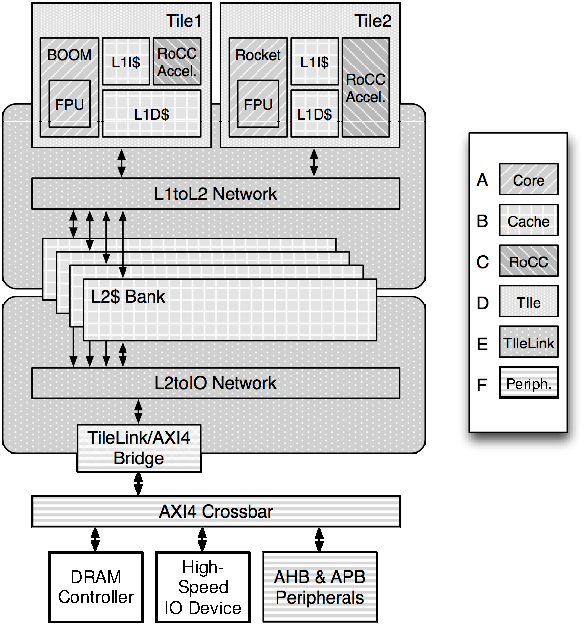
\includegraphics[width=3in]{rcov}
	\caption{Overview of the components of RocketChip.\newline\hspace{\linewidth}\source{Image taken from~\cite{rcgen}}.}
	\label{rcov}
\end{figure}
%}}}
The UCB currently developes three lines of RISC-V processors, Sodor, Rocket and Boom.
Sodor is a collection of simple processors for use in lectures, Rocket is a scalar in-order processor for personal applications and Boom is a superscalar out-of-order processor for high performance applications.
All three are written in Chisel (Creating Hardware in a Scala Embedded Language), a hardware description language --as the name implies-- embedded in Scala.
Chisel allows compilation into three distinct target formats, the first of which is a cycle accurate \CC/ model for fast simulation and software development, the other targets are verilog code aimed at implementation in an FPGA or ASIC\@.
For Rocket and Boom there is a generator framework that can create a whole parametrised system around the processor cores, called RocketChip.
It will create one or more Rocket, Boom or custom cores, surround it with caches, optionally an FPU and accelerators to form one or more [compute-]tiles. Then the tiles are connected to a TileLink network. The CPU is finished by adding TileLink to AXI4 converters to provide a well known bus interface to the outside world. Figure~\ref{rcov} shows a schematic of the generated system.


%{{{
\subsection{General Usage}
The RocketChip is maintained in a Git repository.
To build the default-configuration RocketChip, one only has to clone the repository, build the included GCC toolchain for RISC-V, and run ``\texttt{make}'' as shown in listing~\ref{rcclone}. For building a Boom-chip, the steps are identical except that one also has to checkout the ``\texttt{boom}'' branch of the same repository which then includes the Booms repo as a submodule.

%{{{ RocketChip Build Steps (Listing I)

\begin{table}
	\caption{Build steps for RocketChip.\newline\hspace{\linewidth}Source: Collected from~\cite{rc_github} and~\cite{boom_github}.}
	\begin{subtable}[b]{0.9\linewidth}
		\begin{minted}[fontsize=\small, gobble=3, tabsize=2]{bash}
			# $RC is some place in the file system
			cd $RC
			git clone \
			https://github.com/ucb-bar/rocket-chip.git
			cd rocket-chip
			git checkout boom # Only to build Boom
			git submodule update --init --recursive
		\end{minted}
		\caption{Downloading and initialising.}
		\label{rcclone}
	\end{subtable}
	\begin{subtable}[b]{0.9\linewidth}
		\begin{minted}[fontsize=\small, gobble=3, tabsize=2]{bash}
			cd $RC/riscv-tools
			export RISCV=/where/to/install/toolchain
			export PATH="${PATH}:$RISCV/bin"
			./build.sh # Takes about 45 min
		\end{minted}
		\caption{Building the RSCV-toolchain.}
		\label{rctoolchain}
	\end{subtable}
	\begin{subtable}[b]{0.9\linewidth}
		\begin{minted}[fontsize=\small, gobble=3, tabsize=2]{bash}
			# Substitute ExampleSmallConfig with
			# any available configuration.
			# Use e.g BOOMConfig when building a Boom
			cd $RC/emulator # Build the C++ simulator
			make run CONFIG=ExampleSmallConfig
			cd $RC/vsim     # Create the verilog code
			make -jN CONFIG=ExampleSmallConfig
		\end{minted}
		\caption{Building the SOC and a simulator.}
		\label{rcmake}
	\end{subtable}
\end{table}
%}}}

If the environment variable RISCV is not set to point to a sane installation of the toolchain, the following build steps will fail, so the next part is building the RISCV-toolchain as shown in listing~\ref{rctoolchain}.

\subsection{Configurations}

\subsubsection{Building an existing Configuration}
The makefile has a variable named ``\texttt{CONFIG}'' which is set to the name of a configuration.
A configuration is a set of configuration options that define the generated system.
Available configuration options can be found in \texttt{\$(RC)/src/main/scala/coreplex/Configs.scala}, and include for example:
%{{{ RocketChip config options

\begin{itemize}
	\item What core[s] (Rocket | BOOM | Custom)
	\item \#Tiles/Cores
	\item Cache configuration (Associativity, ECC, replacement policy)
	\item Debug hardware (\#Breakpoints, \#Performance Counters)
	\item What floating point unit
	\item What multiplication and division logic
	\item What atomic instructions
	\item Bootrom
	\item TileLink config
\end{itemize}
%}}}
These options are grouped into different build configurations which can be found in \texttt{\$RC/src/main/scala/rocketchip/Configs.scala}.
Building one of the pre-defined configurations is as simple as setting the \texttt{CONFIG} variable while \texttt{make}-ing the project.
Listing~\ref{rcmake} shows the steps to build the emulator and generate the verilog code for a certain RocketChip configuration.

The generated verilog code is placed into a single file of around 11MB (for \texttt{DefaultConfig}) and includes around 300 verilog modules.
However, the generated code does not only not use any generics like parameterised modules but also involves numerous verbatim copies of the same modules with only the name differing e.g. AsyncResetRegVec\_1..57 (also in \texttt{DefaultConfig}).
Furthermore, the verilog code uses distictive wires for every connection.
While this point-to-point connection scheme probably simplifies the generator code and allows to immediately know which output is driving a certain signal, it renders the code very hard to read as signals can go by many different names although they are electrically connected either directly or through instantiated submodules\footnote{e.g. the clock signal in \texttt{ExampleRocketTop} which is input to the module by the name \texttt{clock}, is connected to (and on another place assigned to) the wire texttt{socBus\_clock}, and assigned to \texttt{AXI4Fragmenter\_1\_clock}, \texttt{AXI4ToTL\_1\_clock}, \texttt{AsyncQueueSink\_1\_1\_clock}, \texttt{AsyncQueueSource\_1\_1\_clock}, \texttt{TLMonitor\_40..52\_clock}, \texttt{TLToAXI4\_2..3\_clock}, \texttt{TLWidthWidget\_2\_clock}, \texttt{bootrom\_TLAtomicAutomata\_clock}, \texttt{bootrom\_TLFragmenter\_clock}, \texttt{bootrom\_TLWidthWidget\_clock}, \texttt{bootrom\_clock}, \texttt{coreplex\_clock}, \texttt{extInterruptXing\_clock}, \texttt{intBus\_clock}, \texttt{l1tol2\_TLSourceShrinker\_clock}, \texttt{l1tol2\_TLWidthWidget\_clock}, \texttt{l2\_clock} and \texttt{peripheryBus\_clock}.}.



%{{{ Config Options (Listing II)

\begin{table}
	\caption{Overview of the configuration system.}
	\begin{subtable}[b]{0.9\linewidth}
		\begin{minted}[fontsize=\small, gobble=3, tabsize=2]{scala}
			class BaseCoreplexConfig
							extends Config ((site, here, up) => {
				case CacheBlockBytes => 64
				case CacheName("L1D") => CacheConfig(
				nSets= 64,
				nWays= 4,
				rowBits= site(L1toL2Config).beatBytes*8,
				nTLBEntries= 8,
				cacheIdBits= 0,
				splitMetadata = false)
				...
			})
			...
			class WithL1ICacheSets(sets: Int)
					extends Config((site, here, up) => {
				case CacheName("L1I") =>
					up(CacheName("L1I"), site).copy(nSets = sets)
			})

			class WithCacheBlockBytes(linesize: Int)
					extends Config((site, here, up) => {
				case CacheBlockBytes => linesize
			})
		\end{minted}
		\caption{Extract of some of the configuration options found in \texttt{\$RC/src/main/scala/coreplex/Configs.scala}.}
		\label{config-options}
	\end{subtable}
	\begin{subtable}[b]{0.9\linewidth}
		\begin{minted}[fontsize=\small, gobble=3, tabsize=2]{scala}
			// Config with 2-way, 32 sets x 64 bytes/block cache
			// tag: 21 bits, index: 5 bits, WS: 4 bits, BS: 2 bits
			class DualCoreConfig2way extends Config(
				new WithNCores(2) ++ new WithL1ICacheWays(2)
				                  ++ new WithL1ICacheSets(32)
				                  ++ new WithCacheBlockBytes(64)
				                  ++ new WithL2Cache
				                  ++ new BaseConfig)

			// Config with 4-way, 64 sets x 32 byts/block cache
			// tag: 21 bits, index: 6 bits, WS: 3 bits, BS: 2 bits
			class DualCoreConfig4way extends Config(
				new WithNCores(2) ++ new WithL1ICacheWays(4)
				                  ++ new WithL1ICacheSets(64)
				                  ++ new WithCacheBlockBytes(32)
				                  ++ new WithL2Cache
				                  ++ new BaseConfig)
		\end{minted}
		\caption{Example of new RocketChip configurations defined in \texttt{\$RC/src/main/scala/rocketchip/Configs.scala}.}
		\label{new-configs}
	\end{subtable}
\end{table}
%}}}
\subsubsection{Creating a new Configuration}
RocketChip configurations are written as scala code and inherit from the \texttt{Config} class defined in \texttt{\$RC/src/main/scala/config/Configs.scala}, which sets up some functionality including the '++' operator that is used to add the configuration options, or one of its child classes which already have some options set.
To evaluate the propagation of different configuration options into the generated verilog code, two new configurations differing in cache associativity and size were created as shown in listing~\ref{new-configs} using the configurations options listed in listing~\ref{config-options}.
\subsubsection{Analysis of configuration propagation}
The instruction cache parameters were chosen for their simple observability. Unlike for example the TileLink configuration options, the cache parameters only affect one verilog module, ICache\_icache, and are relatively simple to check by examining the SRAM memories that are instantiated.
For the 2-way configuration, the core of the cache can be expected to be two 32x21 bit tag SRAMs and two 32x512 bit (32x64 bytes) data SRAMs\footnote{\label{note-width}Or, of course a configuration of smaller width but the same capacity}.
%Likewise one would expect four 64x21 bit tag SRAMs and four 64*256 bit (64*32 bytes) data SRAMs\footnotemark[\ref{note-width}] for the 4-way configuration.
Likewise one would expect four 64x21 bit tag SRAMs and four 64*256 bit (64*32 bytes) data SRAMs\footnoteref{note-width} for the 4-way configuration.

%{{{ Module ICache_icache (Listing III)

\begin{table}
	\caption{Extracts from the generated ICache\_icache Module.}
	\label{srams}
	\begin{subtable}[b]{0.9\linewidth}
		%2-way:
		%tag                   index WS   BS
		%XXXXXXXXXXXXXXXXXXXXX XXXXX XXXX XX
		\begin{minted}[fontsize=\small, gobble=3, tabsize=2]{verilog}
			module ICache_icache(...);
				...
				module tag_array( // Instantiated once
					input  [4:0] RW0_addr,
					input   RW0_en,
					input   RW0_clk,
					input   RW0_wmode,
					input  [20:0] RW0_wdata_0,
					input  [20:0] RW0_wdata_1,
					output [20:0] RW0_rdata_0,
					output [20:0] RW0_rdata_1,
					input   RW0_wmask_0,
					input   RW0_wmask_1
				);
				reg [41:0] ram [31:0];
				...
				module _T_772( // Instantiated twice
					input  [7:0] RW0_addr,
					input   RW0_en,
					input   RW0_clk,
					input   RW0_wmode,
					input  [63:0] RW0_wdata,
					output [63:0] RW0_rdata
				);
				reg [63:0] ram [255:0];
				...
			endmodule
		\end{minted}
		\vspace*{1mm}
		\caption{The instantiated SRAMs for the 2-way configuration.}
		\label{srams-2-way}
	\end{subtable}
	\newline
	\vspace*{7mm}
	\newline
	\begin{subtable}[b]{0.9\linewidth}
		%4-way:
		%tag                   index  WS  BS
		%XXXXXXXXXXXXXXXXXXXXX XXXXXX XXX XX
		\begin{minted}[fontsize=\small, gobble=3, tabsize=2]{verilog}
			module ICache_icache(...);
				...
				module tag_array( // Instantiated once
					input  [5:0] RW0_addr,
					input   RW0_en,
					input   RW0_clk,
					input   RW0_wmode,
					input  [20:0] RW0_wdata_0,
					input  [20:0] RW0_wdata_1,
					input  [20:0] RW0_wdata_2,
					input  [20:0] RW0_wdata_3,
					output [20:0] RW0_rdata_0,
					output [20:0] RW0_rdata_1,
					output [20:0] RW0_rdata_2,
					output [20:0] RW0_rdata_3,
					input   RW0_wmask_0,
					input   RW0_wmask_1,
					input   RW0_wmask_2,
					input   RW0_wmask_3
				);
				reg [83:0] ram [63:0];
				...
				module _T_850( // Instantiated four times
					input  [7:0] RW0_addr,
					input   RW0_en,
					input   RW0_clk,
					input   RW0_wmode,
					input  [63:0] RW0_wdata,
					output [63:0] RW0_rdata
				);
				reg [63:0] ram [255:0];
				...
			endmodule
		\end{minted}
		\vspace*{1mm}
		\caption{The instantiated SRAMs for the 4-way configuration.}
		\label{srams-4-way}
	\end{subtable}
\end{table}
%}}}

Looking at the generated code shown in listing~\ref{srams}, it can be verified, that SRAMS of the expected capacities are indeed created.
However the two and four tag SRAMs are merged into a big single two- and four-port SRAM respectively.
The data SRAMs use a narrower but deeper storage array, providing word-wise access but retaining the correct capacity. The required capacity per cache is the same for both configurations so the same SRAM gets instantiated.
The used SRAM verilog modules get created by the script \texttt{\$RC/vsim/vlsi\_mem\_gen}, which per default, generates behavioural descriptions of the requested SRAMs.
For an actual implementation, this script should be adapted to generate verilog wrappers for actually available SRAM blocks.
Since such an implementation will be forced to always use the next bigger (wider and/or deeper) available SRAMs, it might be beneficial to dimension the cache accordingly to maximise the cache parameters within the used SRAMs.

Looking at the different iterations of generated code, some key modules like the tiles and caches do not seem to change much.
For the rest of the modules, instantiations change considerably when changing the parameters, so hand-writing code to interface to anything within the core except specified interfaces would seem rather unwise.
%}}}

%{{{
\subsection{Interfaces}
%{{{ Figure 2: RocketChip Busses

\begin{figure}%[!t]
	\centering
	\inputimage{image4}
	\caption{The principal busses in the RocketChip. The dashed parts are possible periphery modules and not part of RocketChip.}
	\label{busses}
\end{figure}
%}}}
While the internals of the generated RocketChip vary strongly depending on the configuration options, the external interface is more static.
Save the clock, reset and interrupt lines it consists of the debug interface and some high speed data busses.
Earlier versions of RocketChip used a custom bus interface named Not A Standard Interface (NASTI and NASTI-Lite) for the external busses, but current versions use the Advaced eXtensible Interface (AXI) specified by ARM\cite{axi}.
AMBA and AXI are well known open standards not only with many peripherals readily available as IP but also good support for new development\cite{axi-tools}.

The internal bus system uses TileLink\cite{tilelink}, which is specific to RocketChip and connects the tiles, caches and other core components.
%In standard configuration, the bus consists of two full-duplex, 64-bit data paths.
Using the TileLink and few ancilliarey signals as the only interface for each tile allows easy exchanging of tiles, which is one of the key features allowing the BOOM project to use the RocketChip to create a full processor around their core.
See \cite{rcgen-tutorial} for an overview on how to implement a new tile.

\subsubsection{TileLink}
The physical bus sytem used within the processor is divided into 4 blocks, each with independent synchronisation, data, address, source, size, mask, parameter and opcode signals, implementing two full-duplex paths.
The widths of these signals vary in different parts of the processor. For the Rocket tile in default configuration, there are two TileLink interfaces (io\_cached and io\_uncached) with a width of around 440 each.

TileLink is the cache coherence protocol on top of the physical bus system that connects different agents who participate in a coherent memory model. From TileLinks' point of view, each agent is either a

\begin{description}[\IEEEsetlabelwidth{\texttt{Manager}}\IEEEusemathlabelsep]
	\item[\texttt{Client}] which manipulates data in cache blocks, or a
	\item[\texttt{Manager}] which tracks and controls the access and data flow of the cache blocks.
\end{description}
An agent can also fit into both categories. For example, the L2 cache will appear as a client to caches farther out (or the memory), while managing its clients the L1 caches.



\begin{description}[\IEEEsetlabelwidth{\texttt{Manager}}\IEEEusemathlabelsep]
	\item[\texttt{Client}] which manipulates data in cache blocks, or a
	\item[\texttt{Manager}] which tracks and controls the access and data flow of the cache blocks.
\end{description}




%{{{ Figure 3: TileLink transactions

\begin{figure}%[!t]
	\centering
	\inputimage{image3}
	\caption{An example of TileLink request and release interactions.}
	\label{til-transfer}
\end{figure}
%}}}



\vspace{2cm}
\lipsum


%}}}











%}}}

%\lipsum

%{{{
\section{Conclusion}
The RISCV instruction set architecture is an interesting new player in the field of general purpose ISAs.
It has sparked interest by a broad spectrum of players spanning from research facilities over commercial chip vendors to state-owned defense projects with several implementations in the process of reaching or having reached market-ready status and intensive use in the research field.

Rocket and Boom are open source implementations of RISCV processor cores developed at the university of Berkely, as is RocketChip, a framework written in Chisel that can create processors using Rocket-, Boom- or custom cores.

In this paper, RocketChip was examined, the steps for creating new configurations were laid out, the propagation of the configuration options in Chisel into the generated Verilog code was tested and the relevant internal and external bus interfaces were described.

%Considering the relatively volatile nature of the 





%}}}

\bigskip
%\vfill

%{{{
\begin{thebibliography}{1}
	\bibitem{riscv}
		\url{https://www.youtube.com/watch?v=QTYiH1Y5UV0} At time 17:55
	\bibitem{rcgen}
		Asanovi\'c, Krste/Avizienis, Rimas/Bachrach, Jonathan et at. (2016)\\
		The Rocket Chip Generator.\\
		Technical Report No. UCB/EECS--2016--17, EECS Department, University of California, Berkeley.\\
		\url{http://www2.eecs.berkeley.edu/Pubs/TechRpts/2016/EECS-2016-17.html}\\

	\bibitem{rcgen-tutorial}
		Tutorial for the  Rocket Chip build system. Page 23ff outline how to develop a new tile.\\
		\url{https://riscv.org/wp-content/uploads/2015/01/riscv-rocket-chip-tutorial-bootcamp-jan2015.pdf}

	\bibitem{lowrisc}
		lowRISC: \url{http://www.lowrisc.org/}\\
	\bibitem{sifive}
		SiFive: \url{https://www.sifive.com/}\\
	\bibitem{open-v}
		Open-V: \url{https://www.crowdsupply.com/onchip/open-v}
	\bibitem{pulp}
		Pulp: \url{http://www.pulp-platform.org}\\
		\url{http://iis-projects.ee.ethz.ch/index.php/PULP}
	\bibitem{iid-madras}
		IID Madras: \url{http://rise.cse.iitm.ac.in/shakti.html}\\
	\bibitem{nvidia}
		Nvidia: \url{https://riscv.org/wp-content/uploads/2016/07/Tue1100_Nvidia_RISCV_Story_V2.pdf}\\
	\bibitem{riscv-commercial}
		List of companies presenting commercial implementations of RISC-V at Embedded World 2017\\
		\url{https://riscv.org/2017/03/risc-v-mainstream-ew2017/}
	\bibitem{ucb}
		UC Berkeley: \url{https://www.youtube.com/watch?v=WJndUQssFBg&t=1539s}\\
	\bibitem{rc_github}
		The RocketChip github pages\\
		\url{https://github.com/ucb-bar/rocket-chip}\\
		\url{https://github.com/ucb-bar/project-template}\\

	\bibitem{boom_github}
		The Berkeley Out Of Order Machine github page\\
		\url{https://github.com/ucb-bar/riscv-boom}\\

	\bibitem{tether}
		Github issue about untethered operation of RocketChip\\
		\url{https://github.com/ucb-bar/rocket-chip/issues/434}\\

	\bibitem{axi}
		AMBA® AXI™ and ACE™ Protocol Specification, ARM Limited 2011\\
		\url{https://www.arm.com/products/system-ip/amba-specifications}\\
		Specification, see (A1.1) (requires registration):\\
		\url{http://infocenter.arm.com/help/index.jsp?topic=/com.arm.doc.ihi0022b/index.html}\\
		Specification (download from third party without registration):\\
		\url{http://www.gstitt.ece.ufl.edu/courses/fall15/eel4720_5721/labs/refs/AXI4_specification.pdf}\\

	\bibitem{axi-tools}
		AMBA AXI Accelerated Verification IP (VIP) by Cadence:\\
		\url{https://ip.cadence.com/ipportfolio/verification-ip/accelerated-vip/arm-amba-2/amba-axi-accelerated-vip}\\
		AXI Interconnect support by Xilinx:\\
		\url{https://www.xilinx.com/products/intellectual-property/axi_interconnect.html}\\
		Examplary listing of available IP cores:\\
		\url{https://www.design-reuse.com/sip/amba-axi-c-288/}\\


	\bibitem{tilelink}
		The TileLink Specification, Version 0.3.3\\
		\url{https://docs.google.com/document/d/1Iczcjigc-LUi8QmDPwnAu1kH4Rrt6Kqi1_EUaCrfrk8/pub}\\

\end{thebibliography}
\enlargethispage{-5in}
%}}}


\end{document}
